\chapter{Surgem os Territórios: Simulação, por jhcf}

Este capítulo apresenta os resultados da simulação desenvolvida por Jorge H C Fernandes, cujo planejamento está descrito em \ref{PlanejamentoSimulSurgemOsTerritorios}.

\section{Projeto da Simulação}

As principais características do projeto da simulação foram as seguintes:
\begin{enumerate}
    \item Será usado um modelo de simulação em rede, baseado no código da aplicação ``Virus Network'' disponível no framework de simulação multiagente Python Mesa;
    \item O principal conceito de projeto de simulação usado na construção foi a de que as trocas comerciais entre os territórios em uma rede seguem um modelo de disseminação viral. Ou seja, as trocas comerciais são uma prática, comportamento ou cultura que se espalha sobre os territórios de forma similar à dispersão de uma doença;
    \item Um território ``contaminado'' pela ideia de trocas comerciais pode realizar trocas apenas com outros territórios que também estão contaminados com essa ideia e que se ligam por meio de um canal de relacionamento pre-existente;
    \item A rede de relacionamentos entre os territórios é dirigida, de modo que um território exportador pode enviar suas mercadorias para um território importado, apenas se houver um canal direcionado originado no exportador, e destinado ao importador;
    \item A ocorrência efetiva de trocas entre territórios modifica taxas de fertilidade e mortalidade do território, que são usadas para influência a pirâmide populacional desses;
    \item foram utilizados dados demográficos da população brasileira como base para a definição das pirâmides populacionais dos territórios.
\end{enumerate}

\section{Implementação da simulação}

Os seguintes desafios foram solucionados para o desenvolvimento da simulação:
\begin{enumerate}
    \item Adaptação do framework Mesa para trabalhar com redes dirigidas;
    \item Desenvolvimento do núcleo do modelo de simulação;
    \item Desenvolvimento de um modelo para trabalhar com pirâmide populacional;
    \item Desenvolvimento do servidor; e 
    \item Desenvolvimento dos batches de simulação.
\end{enumerate}

Cada um dos desafios é detalhado a seguir:

\subsection{Adaptação do framework Mesa para trabalhar com redes dirigidas}

O framework Mesa apresenta um exemplo de simulação de contaminação viral em uma rede (grafo), mas o grafo original é não dirigido.
Rozenlitch tentou desenvolver uma versão de Mesa para tratar grafos dirigidos, sem sucesso (\url{https://github.com/rozenlicht/mesa}).
O autor deste relatório usou como base esse fork do Mesa, e fez um novo fork, com várias adaptações ao código, para tratar da questão de grafos dirigidos em mesa, aprimorando o framework. Esse novo fork encontra-se em \url{https://github.com/jhcf/mesa}.

Um sumário das modificações no framework é o seguinte, detalhado em \url{https://github.com/jhcf/mesa/commit/81e461e27b8dd7f3d25ef0bbac08aef3ff6d7d52}:
\begin{enumerate}
    \item  alterado \texttt{mesa/space.py} para criar a classe \texttt{DirectedNetworkGrid (NetworkGrid)}
\item Foi criado o \texttt{mesa/visualization/templates/js/DirectedNetworkModule\_d3.js}, para criar um módulo de rede para tratar com grafos dirigidos.
\item alterado \texttt{mesa/visualization/modules/NetworkVisualization.py}, para rotear o uso da nova função javascript "directed\_d3".
\end{enumerate}

Com as mudanças no framework, envolvendo 174 adições de linha e 3 remoções, foi possível desenvolver uma nova versão do exemplo Virus Directed, adaptado os códigos de:
\begin{enumerate}
\item \texttt{mesa/examples/virus\_on\_network\_directed/virus\_on\_network\_directed/model.py}; e
\item \texttt{
	mesa/examples/virus\_on\_network\_directed/virus\_on\_network\_directed/server.py
}
\end{enumerate}
Na adaptação do exemplo foram feitas 18 adições e 11 remoções de linhas, detalhadas em  \url{https://github.com/jhcf/mesa/commit/0abce10e315f3e3b33ac2912d6f4f43a819f5348}.

Com o aprimoramento do framework Mesa, foi possível fazer o modelo e o servidor para o simulador dos territórios, disponível a partir do diretório  \url{https://github.com/jhcf/Comput-Experim-20202/tree/main/labs/ce20211/surgem_os_territorios}, e descrito a seguir.

\subsection{Desenvolvimento do núcleo do modelo de simulação \textbf{Surgem os Territórios}}

O núcleo da simulação \textbf{Surgem os Territórios} está no módulo \texttt{territorio/model.py}, em \url{https://github.com/jhcf/Comput-Experim-20202/blob/main/labs/ce20211/surgem_os_territorios/territorio/model.py}, nas classes \texttt{NetworkOfTerritories(Model)} e \texttt{TerritoryAgent(Agent)}, descritas a seguir:
\begin{description}
\item [\texttt{NetworkOfTerritories(Model)}]
representa o modelo central da simulação que é uma rede de territórios, definida por um grafo dirigido simples, cujas arestas são canais dirigidos que promovem atividades de troca de exportação e importação, e cujos nós são os agentes, os territórios.  
\item [\texttt{TerritoryAgent(Agent)}] representa um núcleo populacional urbano, uma cidade, de onde podem surgir as universidades e centros de pesquisa. 
\end{description}

O núcleo da simulação é ainda apoiado por uma classe de nome \texttt{Brazilian\-Populational\-Pyramid}, cujas instâncias representam a pirâmide populacional de cada território, e que encapsulam várias funções para modelagem a evolução da população ao longo dos anos. Essa classe tem como base a atual pirâmide populacional brasileira, segundo os dados do IBGE relativos ao ano de 2019.
O código completo desse classe pode ser visto em \url{https://github.com/jhcf/Comput-Experim-20202/blob/main/labs/ce20211/surgem_os_territorios/territorio/BrazilianPopulationalPyramid.py}.

A seguir são apresentados e comentados alguns dos trechos de código mais relevantes das classes que formam o núcleo do modelo de simulação.

\subsubsection{Bibliotecas usadas no modelo}


\lstinputlisting[language=Python,numbers=left,caption={Importações iniciais do modelo de simulação},firstnumber=2, firstline=2, lastline=16,label={jhcf:model:imports}]
{labs/ce20211/surgem_os_territorios/territorio/model.py}

De acordo com o trecho de código na listagem \ref{jhcf:model:imports}, presentam-se as principais dependências do modelo, sendo algumas delas:
\begin{description}
\item [networkx] Para trabalhar com grafos, de vários tipos, inclusive grafos aleatórios e livres de escala;
\item [random] para trabalhar com números aleatórios, e várias distribuições de frequência, inclusive exponencial;
\item [mesa, mesa.time, mesa.datacollections, mesa.space] para usar as facilidades de simulação multiagente desse framework;
\item [networkx.algorithms.communicability\_alg] para obter métricas de comunicabilidade entre os territórios na rede;
\item [BrazilianPopulationalPyramid] para usar uma pirâmide populacional específica para cada território, modelada pela pirâmide populacional brasileira.
\end{description}.

\subsubsection{Principais estados dos territórios do modelo}

\lstinputlisting[language=Python,numbers=left,caption={Enumerações para modelar os estados econômicos e fisiográficos dos territórios},firstnumber=18,firstline=18, lastline=71,label={jhcf:model:states}]
{labs/ce20211/surgem_os_territorios/territorio/model.py}

Cada território criado possui parâmetros para modelar 
o seu estado econômico de realização de trocas comerciais com outros territórios (TradingState), que varia conforme uma das três enumerações nas linhas 15 a 17 da listagem \label{jhcf:model:states}. O TradingState de um território é variável, e é o principal determinante de sua capacidade de realizar trocas, que impacta outros elementos do estado do Território, especialmente a sua população e os canais de troca com outros territórios.

Os parâmetros fisiográficos de solo e clima são fixos, e ainda não estão integrados ao modelo da simulação.

\subsubsection{Propriedades complexas do modelo}

\lstinputlisting[language=Python,numbers=left,caption={Funções que calculam propriedades complexas do modelo em um determinado instante de tempo},firstnumber=72,firstline=72, lastline=122,label={jhcf:model:complex:properties}]
{labs/ce20211/surgem_os_territorios/territorio/model.py}

A partir de uma interação simples de troca comercial nos territórios em rede, é esperado que emerjam propriedades complexas da rede, tais como variação da população, ecentricidade da rede, diâmetro, número de componentes fortemente conectados no grafo, e transitividade do grafo.
As funções declaradas na listagem \ref{jhcf:model:complex:properties} são declaradas para calcular essas propriedades complexas do modelo em um determinado instante de tempo, visando avaliação da condição final ou intermediária do modelo, após alguns passos de simulação.

\subsubsection{Parâmetros centrais do modelo\label{jhcf:model:parameters}}

\lstinputlisting[language=Python,numbers=left,caption={Parâmetros de construção do modelo},firstnumber=127,firstline=127, lastline=148,label={jhcf:model:constructor:parameters}]
{labs/ce20211/surgem_os_territorios/territorio/model.py}


O construtor do modelo NetworkOfTerritories (\ref{jhcf:model:constructor:parameters}) é um dos métodos mais complexos da simulação, e revela os principais parâmetros que definem a evolução do modelo. Breves comentários sobre cada um desses parâmetros são apresentados a seguir, com indicação de seus valores default:
\begin{description}

\item [num\_nodes=10] define a quantidade de territórios que vai compor a rede, durante toda a simulação;
\item [fraction\_of\_brazilian\_population=1] define a população total aproximada da soma de todos os territórios da rede;
\item[alpha=0.41] Define, para a gênese de um grafo livre de escala (método nx.scale\_free\_graph()), o valor do parâmetro alpha, que descreve a chance (41 \% no caso do parâmetro default) de que durante a criação da rede, um território acrescido à rede - variando de dois vértices até o limite máximo do número de vértices no grafo - se ligue a outro que tenha um grau de entrada (capacidade de importação) elevado. Ou seja, a determina a tendência de um um novo território se vincular para exportar para os importadores;
\item [beta=0.54] Define, para a gênese de um grafo livre de escala, o valor do parâmetro beta, que descreve a chance (54 \% no caso do parâmetro default) de que durante a criação de links adicionais entre os nós da rede, visando torná-lo um grafo livre de escala, os pares de territórios existentes se liguem entre si baseados na força da distribuição de frequência combinada com a força de importação do vértice origem, com a força de exportação do vértice destino. Ou seja, determina a tendência de que os territórios fortemente exportadores se vinculem aos territórios fortemente importadores;
\item [gamma=0.05] Define, para a gênese de um grafo livre de escala (método nx.scale\_free\_graph()), o valor do parâmetro gamma, que descreve a chance (5 \% no caso do parâmetro default) de que durante a criação da rede, um território acrescido à rede - variando de dois vértices até o limite máximo do número de vértices no grafo - se ligue a outro que tenha um grau de saída (capacidade de exportação) elevado. Ou seja, a determina a tendência de um um novo território se vincular para exportar para os exportadores
\item [delta\_in=0.02] Modula o viés geral de escolha dos vértices baseados no grau de entrada (privilegia os importadores);
\item [delta\_out=0.0] Modula o viés geral de escolha dos vértices baseados no grau de saída (privilegia os exportadores);
\item [initial\_trading\_perc=1] proporção inicial de vértices que estão disponíveis para comercialização;
\item [trading\_spread\_chance=0.4] chance de que a ideia de comércio ``contamine'' os demais territórios;
\item [trading\_control\_frequency=0.4] chance de que um território busque controlar o seu ``estado'' de infecção pelo comércio - imposição de barreiras comerciais;
\item [trading\_recovery\_chance=0.3] chance de que um território retorne ao estado de neutro acerca de relações comerciais, após ter sido infectado pelo comércio;
\item [trading\_resistance\_chance=0.5] chance de que um território doravante se recuse a fazer trocas comerciais com os demais infectados;
\item [non\_trading\_decay=0.1] grau de decaimento da força de um canal, caso não seja usado para trocas em uma rodada da simulação,
\item [trading\_revigoration = 0.2] grau de revigoramento de um canal, quando usado para realizar trocas comerciais efetivas entre um par de territórios;
\item [visualizing] Informa se é necessário atualizar o valor da variável size a cada passo, um processo computacionalmente custoso, mas útil apenas se a simulação  está sendo visualizada;
\item [seed] Informa a semente do gerador de números aleatórios que poderá ser usada para fixar a aleatoridade durante o processo de depuração do código. 
\end{description}

\subsubsection{Construindo o grafo do modelo}

\lstinputlisting[language=Python,numbers=left,caption={Construindo o grafo do modelo},firstnumber=157,firstline=157, lastline=189,label={jhcf:model:constructor:graph}]
{labs/ce20211/surgem_os_territorios/territorio/model.py}

A construção do grafo inicial do modelo é uma das partes mais sensíveis da simulação, e descrita em \ref{jhcf:model:constructor:graph}. OS seguintes comentários se apresentam.
\begin{description}
\item [Semente da simulação] declarada na linha 158 da listagem, é usada na geração de números aleatórios. Se fixa em um valor numérico, possibilita que o mesmo grafo inicial seja gerado sempre que forem mantidos os parâmetros, N, alpha, beta, gama e deltas. Se declarado como None então aumenta a variabilidade dos grafos gerados, dificultando ganhar intuição sobre o funcionamento correto do modelo, mas sendo essencial para o processo de experimentação.
\item [Ajuste de alpha, beta, gamma] A soma de alfa, beta e gamma sempre deve ser 1, mas não é possível controlar a entrada de dados na interface do server, de modo que as linhas 160 a 189 da listagem \ref{jhcf:model:constructor:graph} fazem esse ajuste, caso a soma não seja 1;
\item [Conversão de multigrafo para grafo dirigido simples] O grafo gerado na linha 175-176 da listagem \ref{jhcf:model:constructor:graph} é um multigrafo, ou seja, vários arcos podem ser dirigidos de um para outro vértice. As linhas 178 a 185 convertem o multigrafo livre de escala em um grafo simples livre de escala, convertendo a multiplicidade de linhas no atributo weight, que é usado para determinar a força de um canal que liga dois territórios;
\item [Variável G] contém a referência ao grafo que modela a estrutura da rede.
\end{description}

\subsubsection{Modelagem da população dos territórios}

\lstinputlisting[language=Python,numbers=left,caption={jhcf:modelagem da população dos territórios},firstnumber=237,firstline=237, lastline=265,label={jhcf:model:constructor:population}]
{labs/ce20211/surgem_os_territorios/territorio/model.py}

A modelagem da população dos territórios é definida na listagem \ref{jhcf:model:constructor:population}. Os  parâmetros para modelagem da população sã detalhados a seguir:
\begin{description}
\item [Distribuição exponencial de frequência da população] O método expon.rvs - linha 239 - gera uma distribuição de frequência exponencial, que será usada para distribuir a população nos territórios a serem gerados, tendo como base a fração da pirâmide populacional brasileira. Para encontrar essa distribuição utiliza-se os parâmetros scale, loc e size. Detalhes em \url{https://docs.scipy.org/doc/scipy/reference/generated/scipy.stats.expon.html}. 
\item [Distribuição da proporção da população nos vértices] a linha 241 da listagem \ref{jhcf:model:constructor:population} ordena a distribuição de frequência exponencial da maior para a menor proporção, a ser usada na distribuição feita entre as linhas 249 a 261;
\item [Ordenamento dos vértices pelo grau ponderado pelo peso dos canais]
A linha 244 classifica todos os vértices do grafo pelo peso do grau total de cada território (número de canais que um território tem com outros), ponderado pelo peso desses canais.
\item [Fração da população brasileira] a pirâmide populacional usada para distribuição de pessoas nos territórios é uma fração da população brasileira em 2019, como mostra o código da linha 246;
\item [Distribuição da população nos territórios]
As linhas 249 a 261 da listagem criam os agentes Território (representam as cidades, de onde vão surgir as universidades, produtoras de conhecimento), distribuindo a população total (fração da população brasileira) usando a distribuição de frequência exponencial casada conforme o peso dos vértices do grafo - que também tem uma distribuição exponencial de frequência, já que são grafos livres de escala (os vértices centrais vão receber a maior população inicial).
\end{description}

\subsubsection{O coletor de dados do modelo}

\lstinputlisting[language=Python,numbers=left,caption={O código do coletor de dados do modelo},firstnumber=217,firstline=217, lastline=235,label={jhcf:model:data:collector}]
{labs/ce20211/surgem_os_territorios/territorio/model.py}

A cada passo da simulação os seguintes dados são coletados no nível do modelo:
\begin{description}
\item [Trading] Quantidade de territórios que podem fazer trocas comerciais;
\item [Available] Quantidade de territórios disponíveis para serem contaminados com a prática do comércio;
\item [Resistant] Quantidade de territórios indisponíveis para a prática do comércio
\item [TotalPopulation] População total da rede de territórios;
\item [Strongcomponents] Número de componentes fortes no grafo que representa a rede de territórios
\item [Transitivity] Métrica de transitividade (Proporção de triângulos possíveis) do grafo que representa a rede de territórios.
\end{description}

A cada passo da simulação os seguintes dados são coletados no nível dos territórios:
\begin{description}
\item [Population] População do território;
\item [EconomicComplexity] Complexidade econômica do território;
\item [State] Condição de disponibilidade para trocas comerciais;
\item [QtyImporters] Quantidade de importadores com os quais um território se relaciona (out degree);
\item [QtyExporters] Quantidade de exportadores com os quais um território se relaciona (in degree).
\end{description}

A cada passo da simulação esses dados podem ser mostrados em um sistema interativo, ou coletados 
no simulador batch.

\subsubsection{Os passos básicos da simulação}

\lstinputlisting[language=Python,numbers=left,caption={Os passos básicos da simulação no nível do modelo},firstnumber=326,firstline=326, lastline=337,label={jhcf:model:step}]
{labs/ce20211/surgem_os_territorios/territorio/model.py}

Os passos básicos da simulação computacional, no nível do modelo, estão declarados na listagem \ref{jhcf:model:step}.
Cada execução do método step representa a passagem de um ano na rede dos territórios.
A cada ano:
\begin{enumerate}
    \item Conta a quantidade de passos da simulação (linha 328);
    \item É imposto um decréscimo anual na taxa de utilização de todos canais (linha 329);
    \item O escalonador de Mesa é chamado a executar os passos de simulação em cada território (linha 330);
    \item A população global do modelo é calculada a partir da soma da população de cada um dos agentes (331);
    \item Os dados são coletados no coletor de dados (linha 332).
\end{enumerate}

Adicionalmente, a listagem \ref{jhcf:model:step} apresenta o método run\_model (linhas 335 a 337), que recebe como parâmetro a quantidade de passos para a realização de um experimento de simulação.
Esse método é útil na automação de batches de simulação.

\subsubsection{A criação dos territórios}

\lstinputlisting[language=Python,numbers=left,caption={A criação do agente Território},firstnumber=356,firstline=356, lastline=384,label={jhcf:model:agent}]
{labs/ce20211/surgem_os_territorios/territorio/model.py}

A criação de cada agente representante de um território é apresentada na listagem \ref{jhcf:model:agent}, e descrita a seguir:
\begin{description}
\item [unique\_id] Cada território tem um identificador único, que é o mesmo número usado quando da construção do grafo livre de escala, iniciando-se em 0, até num\_nodes;
\item [model] cada agente tem uma referência ao modelo, comum a todos;
\item [initial\_state] O estado inicial de disponibilidade para comercializar é definido pelo modelo;
\item [trading\_spread\_chance] A chance que um território tem para contaminar o outro é fixa, e definida no nível do modelo;
\item [trading\_control\_frequency] A taxa de controle sobre as práticas de comércio é fixa, e definida no nível do modelo; 
\item [trading\_recovery\_chance] A chance de um território perder habilidades com a prática do comércio é fixa, e definida no nível do modelo;
\item [trading\_resistance\_chance] A chance de um território se tornar resistente à prática do comércio é fixa, e definida no nível do modelo
\item [populational\_pyramid] A pirâmide populacional específica do território é definida no nível do modelo;
\item [visualizing] Indica se o tamanho relativo dos vértices deve ser atualizado, tendo em vista que é um processo computacionalmente custoso, desnecessário se está sendo executado um batch de simulações, mas necessário se a execução é visual e interativa;
\item [size = 1] O tamanho inicial de um território no modelo é definido como 1, mas pode ser atualizado conforme a proporção da população do território em relação aos demais territórios da rede, caso a simulação esteja sendo feita visualmente.
\end{description}

\subsubsection{Os passos de simulação no nível do agente}

\lstinputlisting[language=Python,numbers=left,caption={O passo de simulação no nível do agente Território},firstnumber=469,firstline=469, lastline=477,label={jhcf:model:agent:step}]
{labs/ce20211/surgem_os_territorios/territorio/model.py}

A listagem \ref{jhcf:model:agent:step} define o que ocorre com cada território a cada ``ano'' da simulação:
\begin{description}
\item [Crescimento da população] Ocorre anualmente, conforme os parâmetros existentes na pirâmide populacional do território (mortalidade e fertilidade);
\item [Tentar fazer trocas] Se o território está contaminado com a prática do comércio, ele tenta encontrar vizinhos também aptos para fazer trocas (linhas 471-472);
\item [Tentar se recuperar de resistência a comércio] Se o território está resistente ao comércio, tenta voltar a ser susceptível à prática (linhas 473-474;
\item [Exerce controle sobre o comércio] O território - possivelmente por meio da fiscalização do Estado - tenta exercer controle sobre as práticas do comércio livre (linha 475);
\item [Atualiza o tamanho aparente do vértice] Se a simulação está sendo visualizada, o território atualiza o valor de seu tamanho aparente, relativo à população total da rede.
\end{description}

\subsubsection{O processo das trocas comerciais}

\lstinputlisting[language=Python,numbers=left,caption={O processo de trocas comerciais entre os Territórios},firstnumber=408,firstline=408, lastline=435,label={jhcf:model:agent:exchanges}]
{labs/ce20211/surgem_os_territorios/territorio/model.py}

O processo das trocas comerciais entre territórios é modelado na listagem \ref{jhcf:model:agent:exchanges}. Ele basicamente envolve os seguintes passos:
\begin{description}
\item [Exportação] (410-422) Para exportar, um território busca todos os demais com os quais se relaciona por meio de um arco de saída (successors), e que estejam também desejando ou disponíveis para comercializar (linhas 410-415). Se ambos estão interessados a troca ocorre (linha 417-418). Se o vizinho está disponível há uma chance dele ser contaminado com a ideia (419-420);
\item [Importação] Para importar, um território busca todos os demais com os quais se relaciona por meio de um arco de entrada (predecessors), e que estejam também interessados ou disponíveis/susceptíveis para comercializar (424-429). Se ambos estão interessados a troca ocorre (431-432). Se o outro está disponível ou susceptível há uma chance de que a troca ocorra (433-435).
\end{description}

\lstinputlisting[language=Python,numbers=left,caption={Detalhe da importação/exportação},firstnumber=393,firstline=393, lastline=406,label={jhcf:model:agent:export}]
{labs/ce20211/surgem_os_territorios/territorio/model.py}

O método trade\_export\_to detalha as consequências da importação/exportação para os agentes.
\begin{description}
\item [Taxa de utilização do canal] (396) O canal (arco dirigido com peso) que liga dois territórios pode ser usado para exportar (self é a origem do arco) ou importar. O volume dessa troca é parametrizado pela largura ou taxa de utilização do canal;
\item [Alteração na taxa de fertilidade] A taxa de fertilidade dos territórios exportadores pode ser alterada pela prática mais ou menos volumosa de  comércio entre territórios com assimetrias em complexidade econômica. Dado que a taxa de uso de um canal vai até 100, cada troca anual influencia esse valor em até 1\%, para mais ou menos (linha 397);
\item [Assimetria econômica 1 (linhas 398-401)] Se uma economia de grande complexidade (398) exporta muito a sua taxa de fertilidade diminui (399). De outra forma, se reduz a complexidade econômica do importador de baixa complexidade (401).
\item [Assimetria econômica 2 (402-405)] Se uma economia de baixa complexidade (402) exporta muito a sua taxa de fertilidade aumenta (403). De outra forma, se incrementa a complexidade econômica do importador (404-405) já com grende complexidade.
\end{description}


Por fim (406), a taxa de utilização do canal entre os dois territórios é revigorada.
 
\subsection{Desenvolvimento do servidor}

O código do servidor gráfico, para visualização da simulação em uma página web, está disponível em \url{https://github.com/jhcf/Comput-Experim-20202/blob/main/labs/ce20211/surgem_os_territorios/territorio/server.py}.

A figura \ref{fig:SurgemOsTerritoriosServer} apresenta uma visualização da interface do servidor, onde se destacam:
\begin{description}
\item [Ajuste de Parâmetros de Simulação] Conforme já descritos em \ref{jhcf:model:parameters};
\item [Visualização da rede de territórios] (centro da figura) Onde o estado de cada território é definido pelo seu tamanho (população), disponibilidade para realizar trocas comerciais (cor) e relacionamentos dirigidos com outros territórios do modelo;
\item [Alguns parâmetros de observação] Tais como a população total da rede, a média da população etc, permitem ganhar intuição sobre o funcionamento do modelo, e seu ajuste aos dados do mundo real (empírico);
\item [Evolução do estado da comercialização] na parte inferior da interface (parcialmente apresentada).
\end{description}


\begin{figure}
    \centering
    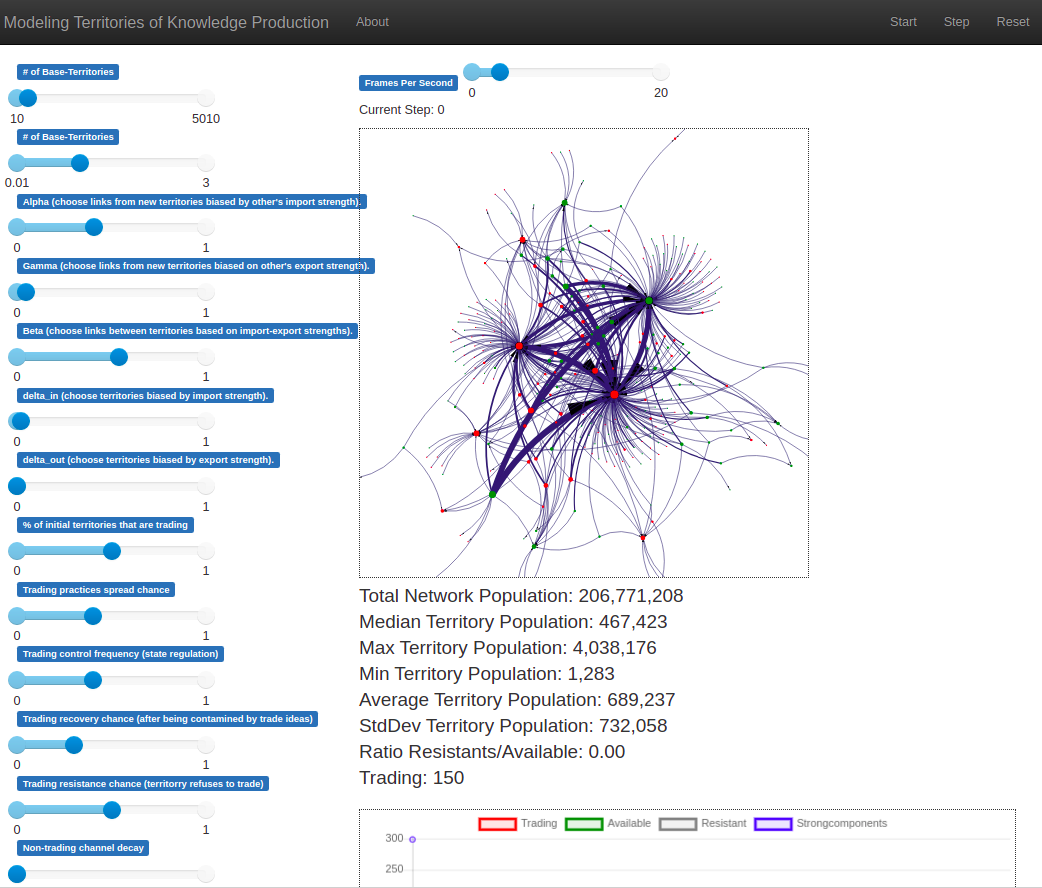
\includegraphics[width=1\textwidth]{experiments/jhcf/ProducaoDaCiencia/Python/SurgemOsTerritoriosServer.png}
    \caption{Aspecto geral de uma simulação no modelo Surgem os Territórios.}
    \label{fig:SurgemOsTerritoriosServer}
\end{figure}


%\lstinputlisting[language=Python,numbers=left,caption="Importações iniciais do modelo de simulação",firstnumber=2,firstline=2, lastline=12,label={jhcf:model:imports}]
%{labs/ce20211/surgem_os_territorios/territorio/server.py}

\subsection{Execução dos batches de simulação (lotes de experimentos)}

Para execução de batches de simulações (lotes de experimentos) foi desenvolvido o método batch\_run, descrito nas listagens \ref{jhcf:model:batch:1}, \ref{jhcf:model:batch:2}, \ref{jhcf:model:batch:3} e \ref{jhcf:model:batch:4}, a seguir.

\subsubsection{Variáveis controladas - mantidas fixas}

\lstinputlisting[language=Python,numbers=left,caption={Variáveis Controladas: Parâmetros fixos para o batch (lote) de simulações},firstnumber=481,firstline=481, lastline=498,label={jhcf:model:batch:1}]
{labs/ce20211/surgem_os_territorios/territorio/model.py}

A listagem \ref{jhcf:model:batch:1} apresenta os parâmetros da simulação que serão mantidos de forma fixa ao longo dos experimentos. Essas são as variáveis controladas, que não serão consideradas como influenciadoras dos efeitos provocados pelas variáveis independentes, a serem descritas na próxima listagem.

Segundo o código da listagem \ref{jhcf:model:batch:1}, as variáveis controladas nesse lote de experimentação são:
\begin{itemize}
\item fraction\_of\_brazilian\_population, representa o tamanho inicial da população a ser simulada. Adotou-se como referência a população do brasil em 1919, em sua relação com a pirâmide populacional relativa a 2019. A ideia é, então, avaliar se o modelo consegue simular a evolução da população brasileira ao longo de cem anos.
\item delta\_in e delta\_out, Variáveis relacionadas com a gênese de uma rede livre de escala, que não serão alteradas.
\item initial\_trading\_perc, trading\_spread\_chance, trading\_control\_frequency, trading\_recovery\_chance, trading\_resistance\_chance e non\_trading\_decay, relativas ao processo de contaminação viral.
\end{itemize}


\subsubsection{Variáveis independentes - manipuladas}

Observe que para que as variáveis independentes passem a ser manipuladas no experimento, basta comentá-las no bloco \ref{jhcf:model:batch:1} e remover os comentários correspondentes do bloco \ref{jhcf:model:batch:2}, e vice-versa.

\lstinputlisting[language=Python,numbers=left,caption={Parâmetros variáveis para o batch (lote) de simulações},firstnumber=500,firstline=500, lastline=512,label={jhcf:model:batch:2}]
{labs/ce20211/surgem_os_territorios/territorio/model.py}

Da maneira como se encontram declarados os parâmetros variáveis da listagem \ref{jhcf:model:batch:2}, podemos dizer que essas são as variáveis independentemente manipuladas do experimento. Como já dito, se as linhas de declaração das mesmas forem comentadas, elas deixam de ser manipuladas, e devem ser declaradas como fixas na listagem \ref{jhcf:model:batch:1}.

As variáveis manipuladas, na listagem \ref{jhcf:model:batch:2}, sofrem variações conforme das declarações de range. Supostamente essas seriam as que exerceriam maior influência sobre a simulação do surgimento dos territórios. Será que isso é verdade? Apenas a realização dos experimentos e a análise dos dados poderá comprovar.

\subsubsection{Configuração do volume de experimentos}

\lstinputlisting[language=Python,numbers=left,caption={Configuração da quantidade de experimentos por caso, e comprimento de cada simulação},firstnumber=514,firstline=514, lastline=545,label={jhcf:model:batch:3}]
{labs/ce20211/surgem_os_territorios/territorio/model.py}

A listagem \ref{jhcf:model:batch:3} apresenta a configuração final dos lotes de experimentos, definindo os seguintes aspectos:
\begin{description}
\item [Quantidade de experimentos por caso] Para cada ajuste de parâmetros fixos e variáveis será executado um número n de experimentos, definido pela variável experiments\_per\_parameter\_configuration. Para que os dados possuam boa significância estatística deve-se realizar, grosso modo, um número grande de experimentos por caso, algo entre 100 e 300. Para se ganhar intuição sobre os efeitos, pode-se iniciar com uma quantidade menor de experimentos, cerca de 10 a 20.
\item [max\_steps\_per\_simulation] Define a quantidade de passos de simulação que serão executados em cada experimento. Conforme o desenho da simulação, a quantidade correta é de 100 passos, um por ano, para simular um século de evolução da população.
\end{description}

Além de definir variáveis de controle e independentes, o experimento deve declarar as variáveis dependentes, ou seja, aquelas cujos efeitos devem ser influenciados pelas variáveis de controle, mas cuja influência maior será determinada pela variação das variáveis independentes.

\subsubsection{Variáveis dependentes - Efeitos gerados}

\lstinputlisting[language=Python,numbers=left,caption={Execução dos experimentos e gravação dos dados coletados},firstnumber=524,firstline=524, lastline=537,label={jhcf:model:batch:4}]
{labs/ce20211/surgem_os_territorios/territorio/model.py}

As variáveis dependentes estão definidas nas linhas 524 a 543. Elas buscam expressar ou representar as consequências potenciais da manipulação das variáveis independentes e do estado fixo das variáveis controladas. Elas são coletadas ao final da simulação, e algumas são relativas ao modelo, mas outras podem ser relativas ao estado dos territórios individuais.
As relativas ao modelo são:
\begin{description}
\item [final\_population] População do território;
\item [number\_trading] quantidade de territórios que estão ativamente tentando comercializar; 
\item [number\_resistant] quantidade de territórios que estão resistentes ao comércio; 
\item [number\_available] quantidade de territórios que estão disponíveis para comercializar; 
\item [network\_number\_strongly\_connected\_components\_not\_unitary] quantidade de componentes fortemente conectados no grafo, com tamanho acima de 1 vértice;
\item [network\_number\_weakly\_connected\_components\_not\_unitary] quantidade de componentes fracamente conectados no grafo;
\item [network\_transitivity] Transitividade da rede
\item [network\_channels\_deceased\_rate] Taxa média de canais de troca que morrem anualmente;
\end{description}

As variáveis dependentes coletadas no nível dos agentes individuais estão declaradas nas linhas 540 a 543.

\subsubsection{Execução dos experimentos e gravação dos dados coletados}

\lstinputlisting[language=Python,numbers=left,caption={Execução dos experimentos e gravação dos dados coletados},firstnumber=546,firstline=546, lastline=556,label={jhcf:model:batch:5}]
{labs/ce20211/surgem_os_territorios/territorio/model.py}

A execução dos experimentos é feita na linha 546 do código na listagem \ref{jhcf:model:batch:5}.
O processo pode ser bastante demorado, dependendo:
\begin{enumerate}
    \item da quantidade de manipulações das variáveis dependentes (multiplica-se os tamanhos das litas de variações para se obter a quantidade básica de interações);
    \item do esforço inerente para realizar os cálculos conforme a magnitude dos valores das variáveis controladas e dependentes;
    \item da quantidade de experimentos realizados para cada combinação de variáveis; e por fim,
    \item da quantidade de passos de simulação executados em cada experimento.
\end{enumerate}

\paragraph{Quantidade de iterações}

A quantidade total de iterações resulta da multiplicação da quantidade 1 (manipulações de variáveis dependentes) pela quantidade de experimentos realizados.

Ao final da execução das iterações, os dados são registrados em duas planilhas distintas, uma para a condição final do modelo em cada uma das interações, e outra para a condição final dos agentes em cada uma das iterações.

\subsection{Análise dos dados da simulação}

Realizados os experimentos, o último passo dessa atividade experimental consistiu de analisar os dados contidos nas planilhas geradas, e fazer as verificações de hipóteses que motivaram a realização do trabalho, concentrada na pergunta: Como surgem os territórios? É possível produzir uma população e rede sintética de territórios que tenha características similares à rede de cidades espalhadas, de onde podem surgir as universidades? 

Para realizar-se essa análise foram comparados os dados gerados no relatório de análise de dados empíricos do IBGE, feito em \ref{jhcf:surgem:os:territorios:analise:dados:empiricos}

Apenas duas análises simples foram realizados em uma primeira série de experimentos, e se encontram no relatório a seguir, baseadas nos arquivos \verb|model_data_iter_10_steps_10_2021-11-05 17:32:12.906885.zip| e \verb|agent_data_iter_10_steps_10_2021-11-05 17:32:12.906885|, localizados em \verb|/experiments/jhcf/ProducaoDaCiencia/Python/experimentos/|.

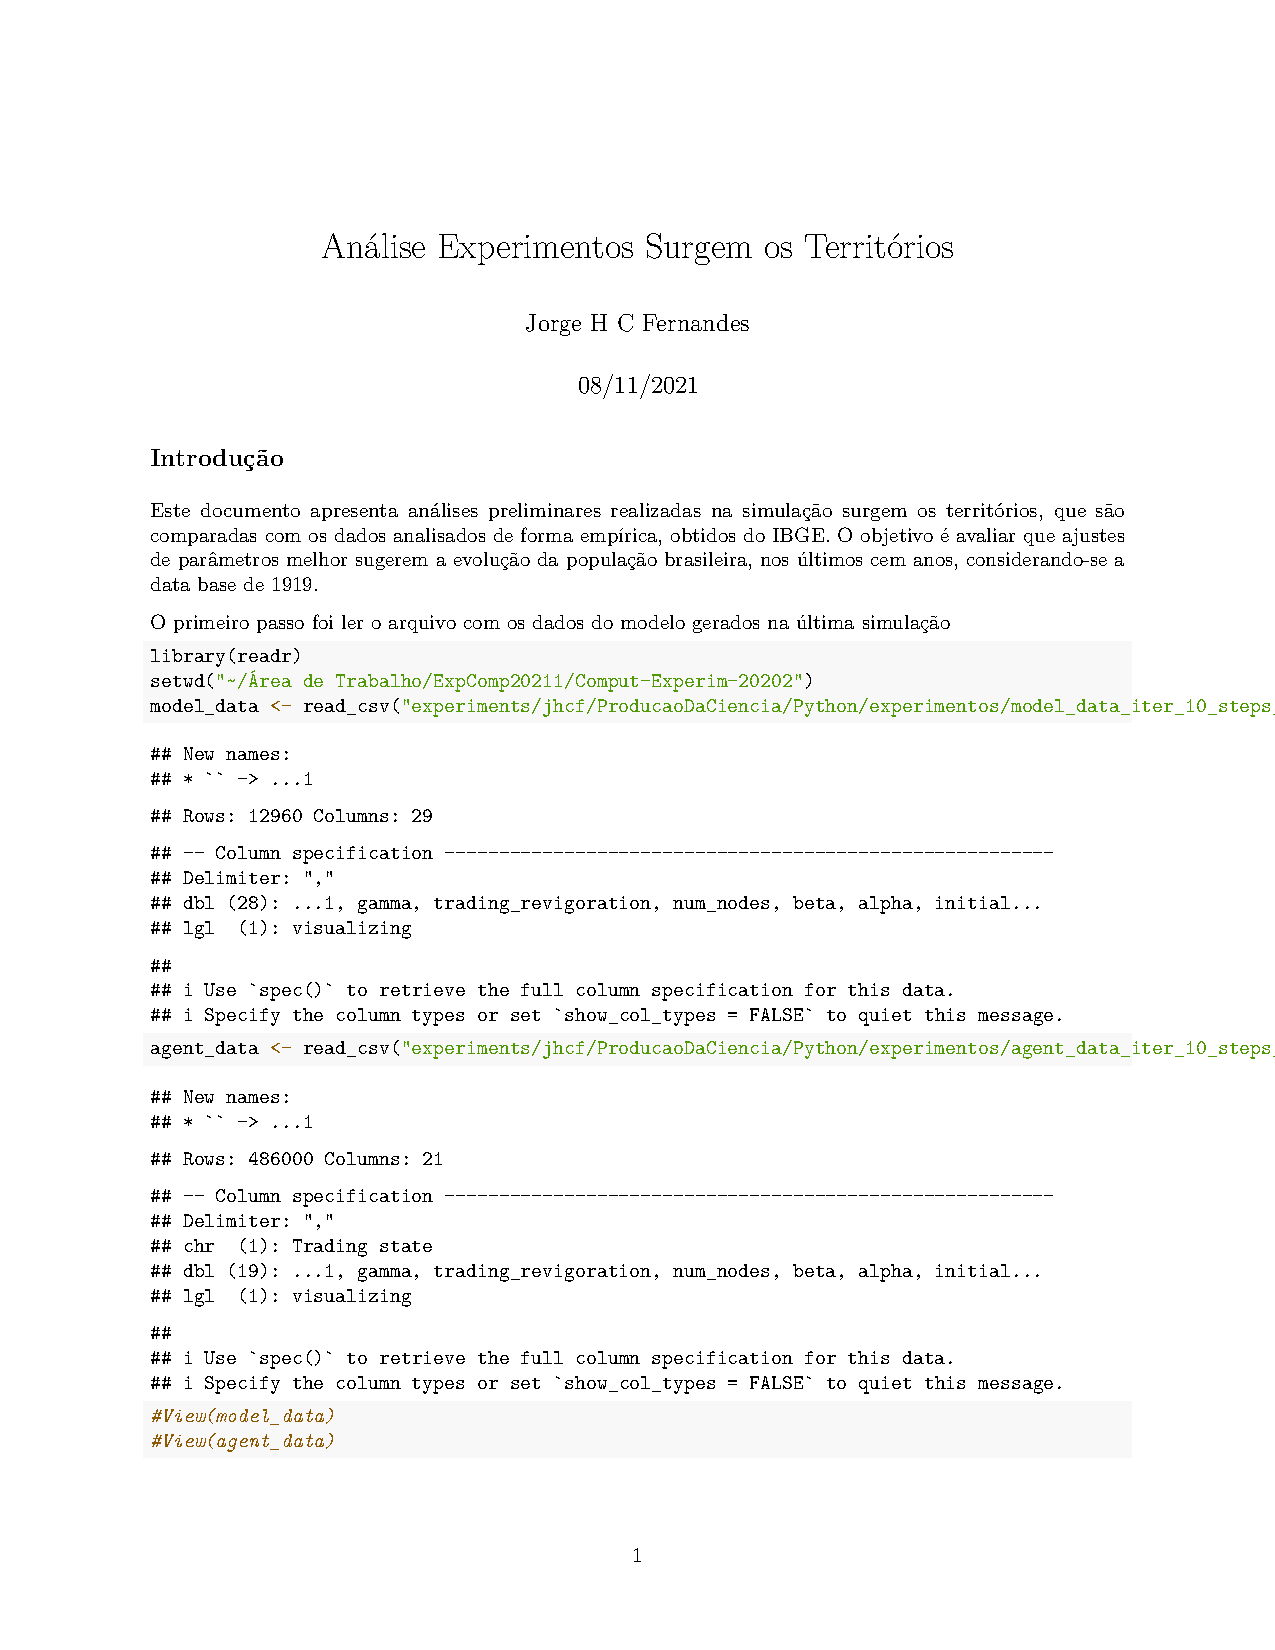
\includepdf[page=-]{experiments/jhcf/ProducaoDaCiencia/R/Territorios/simulacao/AnaliseExperimentosComoSurgemOsTerritorios.pdf}